\documentclass[journal,12pt,twocolumn]{IEEEtran}

\usepackage{setspace}
\usepackage{gensymb}
\singlespacing
\usepackage{amsmath}
\usepackage{amsthm}

\usepackage{mathrsfs}
\usepackage{txfonts}
\usepackage{stfloats}
\usepackage{bm}
\usepackage{cite}
\usepackage{cases}
\usepackage{subfig}

\usepackage{longtable}
\usepackage{multirow}

\usepackage{enumitem}
\usepackage{mathtools}
\usepackage{steinmetz}
\usepackage{tikz}
\usepackage{circuitikz}
\usepackage{verbatim}
\usepackage{tfrupee}
\usepackage[breaklinks=true]{hyperref}
\usepackage{graphicx}
\usepackage{tkz-euclide}

\usetikzlibrary{calc,math}
\usepackage{listings}
    \usepackage{color}                                            %%
    \usepackage{array}                                            %%
    \usepackage{longtable}                                        %%
    \usepackage{calc}                                             %%
    \usepackage{multirow}                                         %%
    \usepackage{hhline}                                           %%
    \usepackage{ifthen}                                           %%
    \usepackage{lscape}     
\usepackage{multicol}
\usepackage{chngcntr}

\DeclareMathOperator*{\Res}{Res}

\renewcommand\thesection{\arabic{section}}
\renewcommand\thesubsection{\thesection.\arabic{subsection}}
\renewcommand\thesubsubsection{\thesubsection.\arabic{subsubsection}}

\renewcommand\thesectiondis{\arabic{section}}
\renewcommand\thesubsectiondis{\thesectiondis.\arabic{subsection}}
\renewcommand\thesubsubsectiondis{\thesubsectiondis.\arabic{subsubsection}}


\hyphenation{op-tical net-works semi-conduc-tor}
\def\inputGnumericTable{}                                 %%

\lstset{
%language=C,
frame=single, 
breaklines=true,
columns=fullflexible
}

\begin{document}

\newcommand{\BEQA}{\begin{eqnarray}}
\newcommand{\EEQA}{\end{eqnarray}}
\newcommand{\define}{\stackrel{\triangle}{=}}
\bibliographystyle{IEEEtran}
\raggedbottom
\setlength{\parindent}{0pt}
\providecommand{\mbf}{\mathbf}
\providecommand{\pr}[1]{\ensuremath{\Pr\left(#1\right)}}
\providecommand{\qfunc}[1]{\ensuremath{Q\left(#1\right)}}
\providecommand{\sbrak}[1]{\ensuremath{{}\left[#1\right]}}
\providecommand{\lsbrak}[1]{\ensuremath{{}\left[#1\right.}}
\providecommand{\rsbrak}[1]{\ensuremath{{}\left.#1\right]}}
\providecommand{\brak}[1]{\ensuremath{\left(#1\right)}}
\providecommand{\lbrak}[1]{\ensuremath{\left(#1\right.}}
\providecommand{\rbrak}[1]{\ensuremath{\left.#1\right)}}
\providecommand{\cbrak}[1]{\ensuremath{\left\{#1\right\}}}
\providecommand{\lcbrak}[1]{\ensuremath{\left\{#1\right.}}
\providecommand{\rcbrak}[1]{\ensuremath{\left.#1\right\}}}
\theoremstyle{remark}
\newtheorem{rem}{Remark}
\newcommand{\sgn}{\mathop{\mathrm{sgn}}}
\providecommand{\abs}[1]{\vert#1\vert}
\providecommand{\res}[1]{\Res\displaylimits_{#1}} 
\providecommand{\norm}[1]{\lVert#1\rVert}
%\providecommand{\norm}[1]{\lVert#1\rVert}
\providecommand{\mtx}[1]{\mathbf{#1}}
\providecommand{\mean}[1]{E[ #1 ]}
\providecommand{\fourier}{\overset{\mathcal{F}}{ \rightleftharpoons}}
%\providecommand{\hilbert}{\overset{\mathcal{H}}{ \rightleftharpoons}}
\providecommand{\system}{\overset{\mathcal{H}}{ \longleftrightarrow}}
	%\newcommand{\solution}[2]{\textbf{Solution:}{#1}}
\newcommand{\solution}{\noindent \textbf{Solution: }}
\newcommand{\cosec}{\,\text{cosec}\,}
\providecommand{\dec}[2]{\ensuremath{\overset{#1}{\underset{#2}{\gtrless}}}}
\newcommand{\myvec}[1]{\ensuremath{\begin{pmatrix}#1\end{pmatrix}}}
\newcommand{\mydet}[1]{\ensuremath{\begin{vmatrix}#1\end{vmatrix}}}
\numberwithin{equation}{subsection}
\makeatletter
\@addtoreset{figure}{problem}
\makeatother
\let\StandardTheFigure\thefigure
\let\vec\mathbf
\renewcommand{\thefigure}{\theproblem}
\def\putbox#1#2#3{\makebox[0in][l]{\makebox[#1][l]{}\raisebox{\baselineskip}[0in][0in]{\raisebox{#2}[0in][0in]{#3}}}}
     \def\rightbox#1{\makebox[0in][r]{#1}}
     \def\centbox#1{\makebox[0in]{#1}}
     \def\topbox#1{\raisebox{-\baselineskip}[0in][0in]{#1}}
     \def\midbox#1{\raisebox{-0.5\baselineskip}[0in][0in]{#1}}
\vspace{3cm}
\title{Assignment 3- Probability and Random Variables}
\author{Songa Kotesh Satvik}
\maketitle
\newpage
\bigskip
\renewcommand{\thefigure}{\theenumi}
\renewcommand{\thetable}{\theenumi}
Download all python codes from 
\begin{lstlisting}
https://github.com/KoteshSatvik/AI1103-Probability_and_Random_Variables/tree/main/Assignment-3/codes
\end{lstlisting}
%
and latex-tikz codes from 
%
\begin{lstlisting}
https://github.com/KoteshSatvik/AI1103-Probability_and_Random_Variables/blob/main/Assignment-3/Assignment3.tex
\end{lstlisting}
\section{\textbf{Gate 2010 (ma) Q:}49}
Let X and Y be continuous random variables with the joint probability density function 
\begin{align}
f\brak{x,y}= 
\begin{cases}
ae^{-2y} & 0<x<y<\infty \\
0 & \text{otherwise}.
\end{cases}   
\end{align}
\\Then $E\brak{X|Y=2}$ is 
\section{\textbf{Solution}}
Given X and Y are two continuous random variables with joint probability density function,
\begin{align}
f\brak{x,y}= 
\begin{cases}
ae^{-2y} & 0<x<y<\infty \\
0 & \text{otherwise}.
\end{cases}   
\end{align}
\begin{figure}[!hbt]
    \centering
    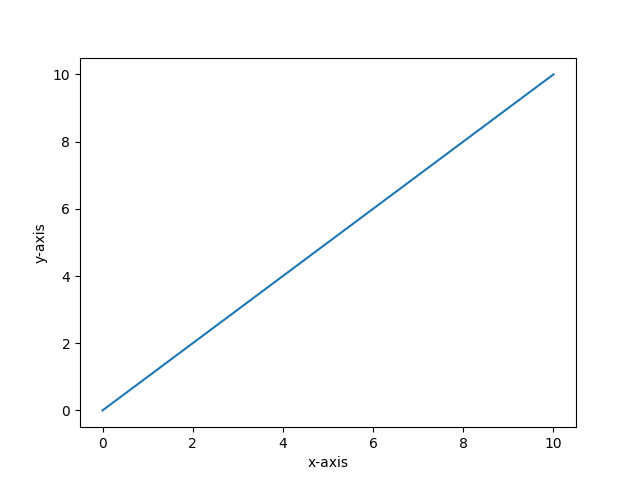
\includegraphics[width=\columnwidth]{Figure_0.png}
    \caption{Graph of x=y}
    \label{Figure_1}
\end{figure}
We know that,\\
$0<x<y<\infty  \implies x<y<\infty \text{ for } 0<x<\infty.$\\ 
Then,
\begin{align}
    f_X\brak{x} &= \int f_{XY}\brak{x,y}dy\\
    &= \int_{x}^{\infty} ae^{-2y}dy\\
    &= \left[ \frac{ae^{-2y}}{(-2)} \right]_{x}^{\infty}\\
    &= \frac{-a}{2}\left[ e^{-2y}\right]_{x}^{\infty}\\
    &= \frac{-a}{2}[0-e^{-2x}]\\
\implies f_X\brak{x} &=
    \begin{cases}
    \frac{a}{2}e^{-2x} & 0 < x < \infty\\
    0 & \text{otherwise}.
    \end{cases}
\end{align}
Similarly,\\
$ 0<x<y<\infty \implies 0<x<y \text{ for } 0<y<\infty$ \\
Then,
\begin{align}
    f_y\brak{y} &= \int f_{XY}\brak{x,y}dx\\
    &= \int_{0}^{y} ae^{-2y}dx\\
    &= ae^{-2y}[x]_{0}^{y}\\
    &= aye^{-2y}\\
\implies f_Y\brak{y} &=
    \begin{cases}
    aye^{-2y} & 0 < y < \infty\\
    0 & \text{otherwise}.
    \end{cases}
\end{align}
%\begin{figure}[ht]
%    \centering
%    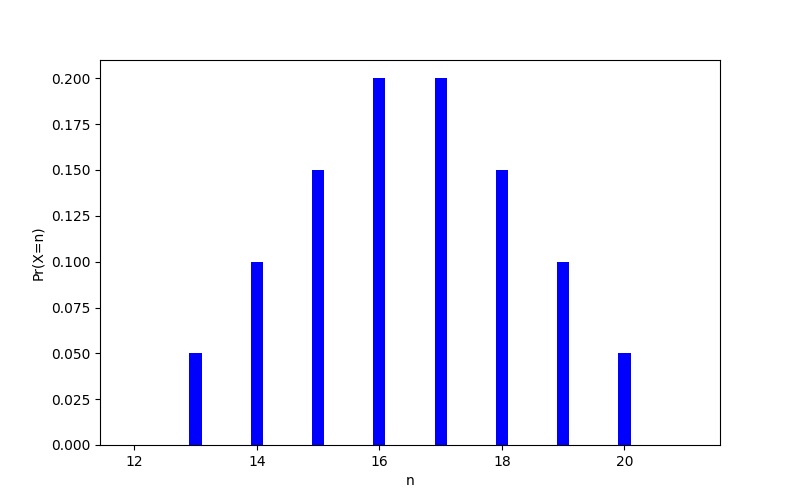
\includegraphics[width=\columnwidth]{Figure_1.png}
%    \caption{Graph of x+y=1}
%    \label{Figure_1}
%\end{figure}
Therefore ,
\begin{align}
    f_{X|Y}\brak{x|y} &= \frac{f_{XY}\brak{x,y}}{f_Y\brak{y}}\\
    & = \frac{ae^{-2y}}{aye^{-2y}}\\
    & = \frac{1}{y}\\
\implies f_{X|Y}\brak{x|y} &=
    \begin{cases}
    \frac{1}{y} & \text{if } 0<x<y<\infty\\
    0 & \text{otherwise}
    \end{cases}
\end{align}
Then, 
\begin{align}
   E\brak{X|Y=y} & =
   \int_{-\infty}^{\infty} (x)f_{X|Y}\brak{x|y}dx\\
    & = \int_{0}^{y}(x)\brak{\frac{1}{y}}dx\\
    & = \frac{1}{y} \int_{0}^{y}(x)dx \\
    & = \frac{1}{y} \left[ \frac{x^2}{2}\right]_{0}^{y}\\
    & = \frac{1}{y}\brak{\frac{y^2}{2}}\\
    & = \frac{y}{2}\\
\implies E\brak{X|Y=y} &= \frac{y}{2}\\
\therefore E\brak{X|Y=2} &= 1
\end{align}
\end{document}